\newpage
\section{Perpeve}
Nesse jogo temos um tabuleiro $5 \times 8$ onde quem chegava no círculo preto tinha direito a pegar um papel da caixa de surpresas. 

\begin{center}
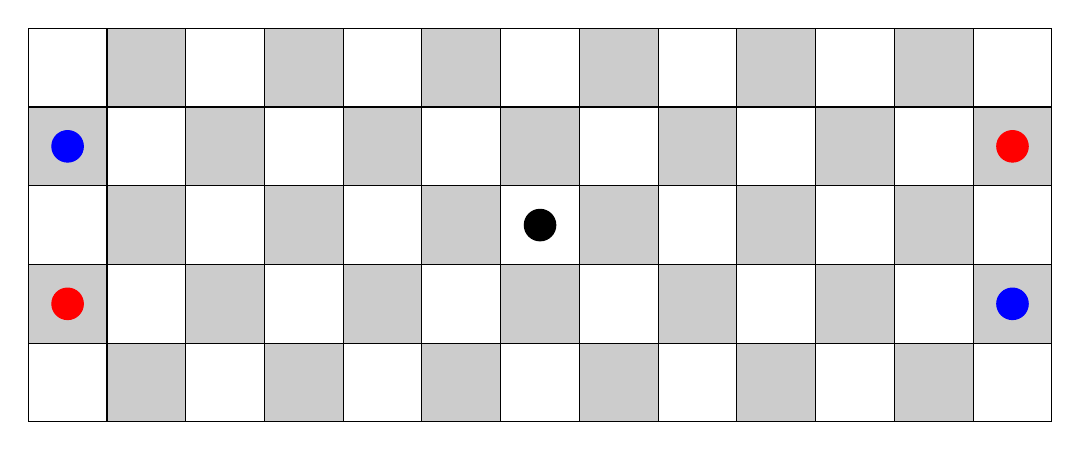
\begin{tikzpicture}
  \def\rows{5}
  \def\cols{13}

  % Desenhar o tabuleiro com padrão xadrez
  \foreach \x in {0,...,12} {
    \foreach \y in {0,...,4} {
      \pgfmathtruncatemacro{\shade}{mod(\x+\y,2)}
      \ifnum\shade=1
        \fill[gray!40] (\x,-\y) rectangle ++(1,-1);
      \else
        \fill[white] (\x,-\y) rectangle ++(1,-1);
      \fi
      \draw (\x,-\y) rectangle ++(1,-1);
    }
  }

  % Círculos pretos CENTRALIZADOS nas casas pretas
  
  \filldraw[blue] (0 + 0.5, -1 - 0.5) circle (0.2);
  \filldraw[red] (0 + 0.5, -3 - 0.5) circle (0.2);
  \filldraw[red] (12 + 0.5, -1 - 0.5) circle (0.2);
  \filldraw[blue] (12 + 0.5, -3 - 0.5) circle (0.2);
  \filldraw[black] (6 + 0.5, -2 - 0.5) circle (0.2);
\end{tikzpicture}
\end{center}

Vamos considerar o tabuleiro como sendo o nosso espaço $S$. Existem dois tipos de jogadores que vivem no mesmo espaço. Os jogadores de um lado, podem se mover apenas duas casas em uma das direções ($\uparrow$ $\downarrow$ $\leftarrow$ $\rightarrow$). Enquanto que o outro lado se moviam apenas duas casas nas direções ($\nwarrow$  $\nearrow$ $\swarrow$ $\searrow$ ). Uma regra interessante nesse jogo é que se o jogador chegasse na parede e ele tivesse mais uma casa para andar, ele iria refletir seu movimento; e caso ele encontrasse um jogador, ele interromperia o movimento. 

Podemos imaginar o movimento desses jogadores como sendo a métrica usada para calcular distâncias. Em vez de darmos regras de movimentos, que tal apenas a regra: um jogador só pode andar dentro da bola fechada de raio $r$ de sua métrica? Para isso, vamos definir as métricas:
\\
\begin{center}
  $M_1(x, y)$ = \begin{cases}
    ;& x = y\\
    $||x - y||_{\infty}$; & x - y \in \{(\pm r, \pm r)\}\\
  r + 1; & \text{caso contrário}
  \end{cases}
\end{center}
\\

\begin{center}
  $M_2(x, y)$ = \begin{cases}
    0; & x = y\\
    $||x - y||_{\infty}$; & x - y \in \{(\pm r, 0), (0, \pm r)\}\\
    r+1; & \text{caso contrário}
  \end{cases}
\end{center}
\\

  Perceba que para $r = 2$, a bola fechada geraria os movimentos dos jogadores. Mas percebi que na realidade está errado, essa métrica ficou circular e não consegui pensar em um meio de resolver, não ainda ao menos. Mas acho que é assim possível definir uma métrica onde fixo uma distância $d(x,y)=2$ e falo que os jogadores só podem andar esas distância. Ademais, gostei bastante da atividade 

\section{Jogo da Memória}

Nesse jogo vimos como era a relação entre a métrica e os pontos que tem uma distância fixa $r$ no espaço, como por exemplo, a euclidiana gerando um círculo que conhecemos usualmente, e o binário gerando o $\mbb{R}^2 - \{(0,0)\}$. Inicialmente eu achei que estavam gerando bolas, mas depois percebi que o intuito era representar pontos que estão a uma mesma distância.

\section{Complete as lacunas}

Nesse jogo ficou em ordem: Note que $a \leq |a|, \forall a \in \mbb{R}$. De modo similar, $b \leq |b|, \forall b \in \mbb{R}$. Assim, somando ambas, temos que $a + b \leq |a| + |b|$. Por outro lado $-a \leq |a|$ e $-b \leq |b|$. Assim, $-a -b \leq|a| + |b|$ implicando que $-(|a| + |b|)\leq a + b$, portanto $-(|a| + |b|) \leq a + b \leq |a| + |b|$

\section{Chat}
Eu consegui compreender quando vi a comapração de $d_1 e d_{\infty}$ e $d_2 e d_{\infty}$, mas não cheguei a pensar em um método razoável para comparar com $d_1 e d_2$ antes do tempo estabelecido. Passei mais tempo tentando entender como o GPT fez algumas implicações do nada. Então nem passou pela minha cabeça em tentar usar a desigualdade de Cauchy-Scharwz  
